\documentclass[ignorenonframetext,xcolor=dvipsnames]{beamer}
\setbeamertemplate{caption}[numbered]
\setbeamertemplate{caption label separator}{:}
\setbeamercolor{caption name}{fg=normal text.fg}
\usepackage{amssymb,amsmath}
\usepackage{ifxetex,ifluatex}
\usepackage{fixltx2e} % provides \textsubscript
\usepackage{lmodern}
\ifxetex
  \usepackage{fontspec,xltxtra,xunicode}
  \defaultfontfeatures{Mapping=tex-text,Scale=MatchLowercase}
  \newcommand{\euro}{€}
\else
  \ifluatex
    \usepackage{fontspec}
    \defaultfontfeatures{Mapping=tex-text,Scale=MatchLowercase}
    \newcommand{\euro}{€}
  \else
    \usepackage[T1]{fontenc}
    \usepackage[utf8]{inputenc}
      \fi
\fi
% use upquote if available, for straight quotes in verbatim environments
\IfFileExists{upquote.sty}{\usepackage{upquote}}{}
% use microtype if available
\IfFileExists{microtype.sty}{\usepackage{microtype}}{}
\usepackage{url}
\usepackage{graphicx}
\makeatletter
\def\maxwidth{\ifdim\Gin@nat@width>\linewidth\linewidth\else\Gin@nat@width\fi}
\def\maxheight{\ifdim\Gin@nat@height>\textheight0.8\textheight\else\Gin@nat@height\fi}
\makeatother
% Scale images if necessary, so that they will not overflow the page
% margins by default, and it is still possible to overwrite the defaults
% using explicit options in \includegraphics[width, height, ...]{}
\setkeys{Gin}{width=\maxwidth,height=\maxheight,keepaspectratio}

% Comment these out if you don't want a slide with just the
% part/section/subsection/subsubsection title:
\AtBeginPart{
  \let\insertpartnumber\relax
  \let\partname\relax
  \frame{\partpage}
}
\AtBeginSection{
  \let\insertsectionnumber\relax
  \let\sectionname\relax
  \frame{\sectionpage}
}
\AtBeginSubsection{
  \let\insertsubsectionnumber\relax
  \let\subsectionname\relax
  \frame{\subsectionpage}
}

\setlength{\parindent}{0pt}
\setlength{\parskip}{6pt plus 2pt minus 1pt}
\setlength{\emergencystretch}{3em}  % prevent overfull lines
\setcounter{secnumdepth}{0}
%% Options for beamer presentation using pandoc

% Theme
\usetheme[width=0cm]{Hannover}
\usecolortheme[named=MidnightBlue]{structure}
\usecolortheme{orchid}

% Set packages
\usepackage[T1]{fontenc} 
\usepackage{tgadventor}

%% Beamer options
\makeatletter
\setbeamertemplate{sidebar canvas left}{}
\makeatother
\beamertemplatenavigationsymbolsempty %remove navigation bars on the bottom
\setbeamercolor{block body}{bg=white}
\setbeamertemplate
{frametitle}
{
  \begin{flushleft}
        \textbf{\insertframetitle}
  \end{flushleft}
}

\title{Know your data and how to analyze it correctly: Statistical assumptions}
\author{Daiva \& Luke}
\date{2015-01-30}

\begin{document}
\frame{\titlepage}

\begin{frame}{Welcome to our Statistical Assumptions workshop}

\begin{block}{Purpose:}

To teach the statistical assumptions of linear regression and show how
you test data to see if they satisfy the assumptions. Knowing how to
check these assumptions is part of ``best practices'' in data analysis.

\end{block}

\begin{block}{Significance:}

It is very important to check that your data satisfies linear regression
assumptions. If your data does not meet these criteria, the use of
linear regression is inappropriate. Other methods can be used,
but\ldots{}

\end{block}

\end{frame}

\begin{frame}{Caveat (again): We aren't here to teach statistics}

Need help with stats? Use these resources!

\begin{itemize}
\item
  U of T Statistical Consulting Services
  (\href{http://www.utstat.toronto.edu/wordpress/?page_id=25}{click
  here})
\item
  \url{http://www.stackoverflow.com}
\item
  \url{http://stats.stackexchange.com}
\item
  Helpful statistical tests flowchart (PDF on GitHub)
\item
  Very helpful webpage on regression diagnostics:
  \url{http://www.ats.ucla.edu/stat/sas/webbooks/reg/chapter2/sasreg2.htm}
  (Note: Goes into much more detail than what is covered in this
  workshop)
\end{itemize}

\end{frame}

\begin{frame}{Notes and help during this workshop}

Go to this website:

\url{https://etherpad.mozilla.org/dnsWorkshops}

\end{frame}

\begin{frame}{Linear Regression}

\begin{itemize}
\item
  Used to test associations between independent and dependent variables
\item
  Based on a linear relationship: \(y = X\beta + \varepsilon\)

  \begin{itemize}
  \itemsep1pt\parskip0pt\parsep0pt
  \item
    y = dependent variable(s)
  \item
    \(\beta\) = slope
  \item
    X = independent variable
  \item
    \(\varepsilon\) = error, or residual, terms
  \end{itemize}
\end{itemize}

\end{frame}

\begin{frame}{Some Linear Regression Assumptions}

\begin{itemize}
\item
  Model is good (i.e.~linear relationship between predictors and outcome
  variable)
\item
  Residuals\footnote<.->{Residual (aka the error term) = observed -
    expected} have a normal distribution
\item
  Residuals are homoscadastic (have equal/constant variance)
\end{itemize}

\end{frame}

\begin{frame}{Other Checks to Ensure Appropriate Model}

\begin{itemize}
\item
  Check for collinearity (predictors that are highly linearly related --
  may result in inaccurate estimates of regression coefficients)
\item
  Check for influence (i.e.~outliers)
\end{itemize}

\end{frame}

\begin{frame}{Brief aside: assumptions/diagnostics we are not covering
in this workshop}

\begin{itemize}
\item
  Independence (residuals of one observation are not associated with
  residuals of another)
\item
  Errors in variables (predictor variables are measured without error)
\item
  Very helpful webpage on regression diagnostics that covers these:
  \url{http://www.ats.ucla.edu/stat/sas/webbooks/reg/chapter2/sasreg2.htm}
\end{itemize}

\end{frame}

\begin{frame}{How to check assumptions}

\begin{itemize}
\item
  Model fit: Plot residuals vs.~predicted fit (check pattern)
\item
  Distribution of residuals: Normal probability plot
\item
  Variance of residuals: Plot residuals vs.~predicted fit (check spread
  of points)
\end{itemize}

\end{frame}

\begin{frame}[fragile]{Model fit}

\begin{verbatim}

    * Run a scatter plot;
    proc sgplot data=sashelp.fish;
        scatter x=weight y=length1;
    run;
\end{verbatim}

\end{frame}

\begin{frame}{Model fit}

\begin{figure}[htbp]
\centering
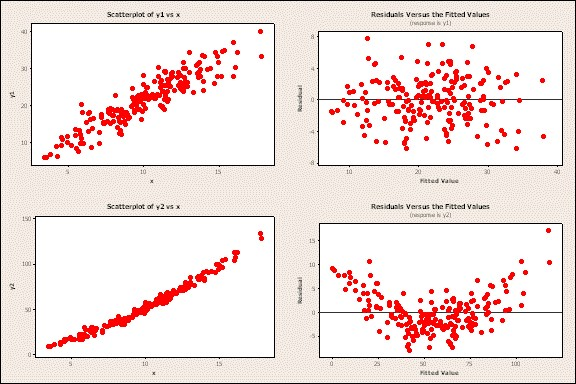
\includegraphics{img/modelFit.jpg}
\caption{}
\end{figure}

\end{frame}

\begin{frame}[fragile]{Residual distribution}

\begin{verbatim}
    * Run a linear regression model and output the ;
    * residual and predicted terms to a new dataset;
    proc reg data=sashelp.fish;
        model height=weight;
        output out=resid residual=r predicted=fit;
    run;
    quit;

    * Create a plot of the new output dataset;
    goptions reset=all;
    proc univariate data=resid normal;
        var r;
        qqplot r / normal(mu=est sigma=est);
    run;
\end{verbatim}

\end{frame}

\begin{frame}{Residual distribution}

\begin{figure}[htbp]
\centering
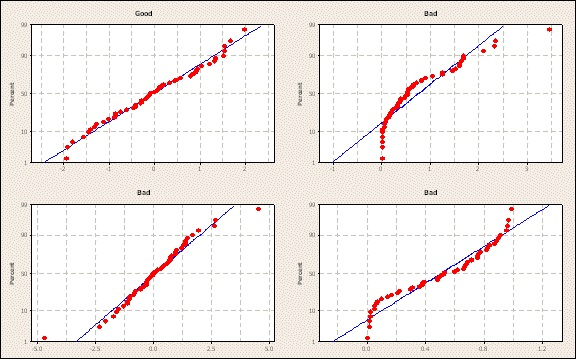
\includegraphics{img/residNorm.jpg}
\caption{}
\end{figure}

\end{frame}

\begin{frame}[fragile]{Residual variance}

\begin{verbatim}
    proc reg data=sashelp.fish;
        model height=weight;
        plot r.*p.;
    run;
    quit;
\end{verbatim}

\end{frame}

\begin{frame}{Residual variance}

\begin{figure}[htbp]
\centering
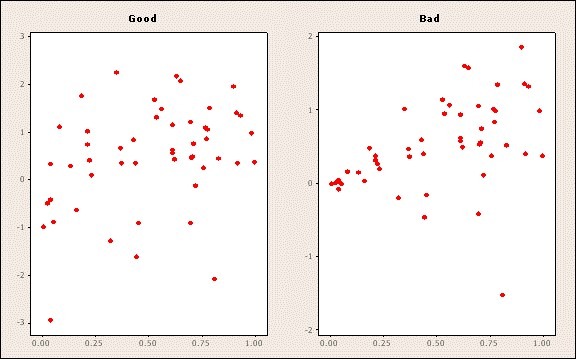
\includegraphics{img/residVar.jpg}
\caption{}
\end{figure}

\end{frame}

\begin{frame}[fragile]{What do you do if your data does not meet these
assumptions?}

\begin{itemize}[<+->]
\itemsep1pt\parskip0pt\parsep0pt
\item
  Try transforming the data (log, square root)
\end{itemize}

\begin{verbatim}
    data new;
        set sashelp.fish;
        logWt = log(Weight);
        run;
\end{verbatim}

\begin{itemize}[<+->]
\itemsep1pt\parskip0pt\parsep0pt
\item
  Use a non-parametric statistical test if can not obtain normal
  distribution of residuals after attempting a transformation
\end{itemize}

\end{frame}

\begin{frame}[fragile]{Collinearity}

\begin{itemize}
\itemsep1pt\parskip0pt\parsep0pt
\item
  What is it? Two or more predictors in a model that are moderately to
  highly correlated with one another (e.g.~BMI and body weight)
\end{itemize}

\pause

\begin{itemize}
\itemsep1pt\parskip0pt\parsep0pt
\item
  Check VIF (variance inflation factor)

  \begin{itemize}
  \itemsep1pt\parskip0pt\parsep0pt
  \item
    OR Check tol (tolerance = 1/vif)
  \end{itemize}
\end{itemize}

\begin{verbatim}
    proc reg data=sashelp.fish;
        model height = weight length / vif tol;
    run;
    quit;
\end{verbatim}

\begin{itemize}
\itemsep1pt\parskip0pt\parsep0pt
\item
  VIF \textgreater{} 10 or tol \textless{} 0.1 suggest collinearity is
  present
\end{itemize}

\end{frame}

\begin{frame}[fragile]{Influence}

\begin{itemize}[<+->]
\itemsep1pt\parskip0pt\parsep0pt
\item
  Make a scatterplot of all observations
\end{itemize}

\begin{verbatim}
    proc gplot data=sashelp.fish;
        plot height*weight=1 / vaxis=axis1;
    run;
    quit;
\end{verbatim}

\begin{itemize}[<+->]
\itemsep1pt\parskip0pt\parsep0pt
\item
  Do a visual check for extreme observations
\end{itemize}

\begin{itemize}[<+->]
\itemsep1pt\parskip0pt\parsep0pt
\item
  OR proc univariate will output extreme observations
\end{itemize}

\begin{itemize}[<+->]
\itemsep1pt\parskip0pt\parsep0pt
\item
  Observation is ``influential'' if removing it substantially changes
  the estimate of coefficients (sometimes! exception: genetics--extreme
  observations may be hyper/hypo-responders)
\end{itemize}

\end{frame}

\begin{frame}{Main Exercise}

\begin{enumerate}
\def\labelenumi{\arabic{enumi}.}
\itemsep1pt\parskip0pt\parsep0pt
\item
  Download the Statistical Tests Flowchart from GitHub (.pdf).
\item
  Use the SAS help dataset fish (\texttt{sashelp.fish}) or your own
  data.
\item
  Perform assumptions check using your statistical analysis software.
\item
  Write a report summary of results for the assumptions we covered and
  conclude whether or not linear regression is appropriate for this
  data.
\item
  Check for collinearity and influence.
\end{enumerate}

\end{frame}

\end{document}
